\providecommand{\main}{../../..}
\documentclass[\main/dresen_thesis.tex]{subfiles}

\begin{document}
  \section{MARIA}\label{ch:lss:maria}
    \begin{figure}[ht]
      \centering
      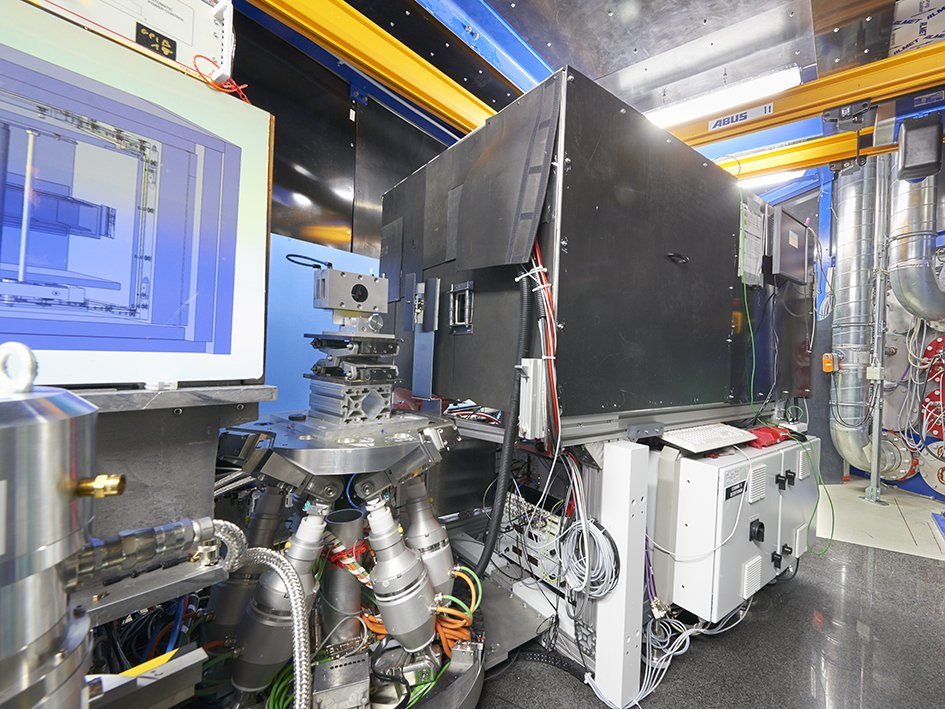
\includegraphics[width=0.7\textwidth]{appendix_instruments_maria}
      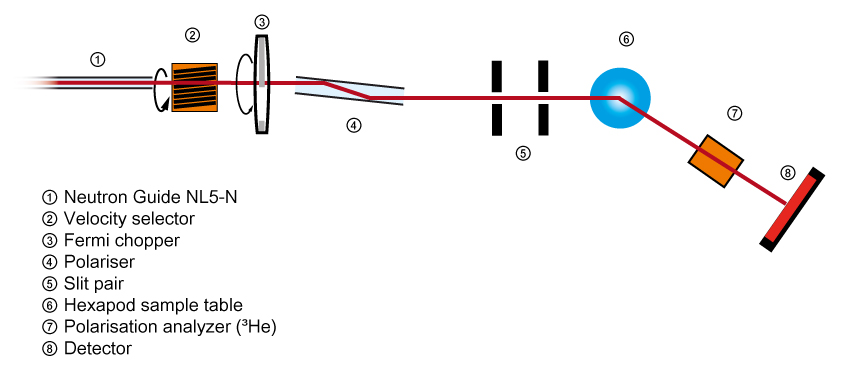
\includegraphics[width=0.7\textwidth]{appendix_instruments_mariaSetup}
      \caption{\label{fig:lss:maria}The MARIA instrument at Heinz Maier-Leibnitz Zentrum used for (polarized) neutron reflectometry and grazing incidence small angle neutron scattering \cite{Heinz_2015_Maria}.}
    \end{figure}

    The MAgnetic Reflectometer with high Incident Angle (MARIA) at the Heinz Maier-Leibnitz Zentrum is a neutron reflectometer with polarisation analysis operated by the J\"ulich Center for Neutron Science (JCNS) \cite{Heinz_2015_Maria}.
    It is designed to study samples with a layer thickness of $0.3 - 30 \unit{nm}$ and can also be used in GISANS mode to study lateral structures on the order of $3 - 300 \unit{nm}$.
    The optimal neutron flux is achieved at $\lambda \approx 4.5 \angstrom$.
\end{document}